% "Compositing shaders in X3D" by Michalis Kamburelis,
% for Web3D 2011.
%
% If accepted, this will be © Copyright 2011 by ACM, Inc.
% See http://www.acm.org/publications/policies/copyright_policy
%

%% Template stuff begins here ------------------------------------------------

\documentclass{acmsiggraph}                     % final
%\documentclass[annualconference]{acmsiggraph}  % final (annual conference)
%\documentclass[review]{acmsiggraph}            % review
%\documentclass[widereview]{acmsiggraph}        % wide-spaced review
%\documentclass[preprint]{acmsiggraph}          % preprint

\usepackage[scaled=.92]{helvet}
\usepackage{times}
\usepackage{graphicx}
\usepackage{parskip}
\usepackage[labelfont=bf,textfont=it]{caption}
\onlineid{1010} %% I think this doesn't matter

%% Template stuff ends here ------------------------------------------------

% This is really the only sensible way to make breaking of monospace text
% (everything inside \texttt, including (but not limited) to urls).
% Otherwise, the monospace text flows outside of the column all over the place.
\sloppy

\usepackage{needspace}

%% For href
\usepackage{ifpdf}
\ifpdf
  \usepackage[pdftex]{hyperref}
\else
  \usepackage[hypertex]{hyperref}
\fi

%% Put float in a nice box,
%% http://en.wikibooks.org/wiki/LaTeX/Floats,_Figures_and_Captions
\usepackage{float}
\floatstyle{boxed}
\newfloat{mycodecore}{H}{listofmycode}
\floatname{mycodecore}{}

% Fix mycodecore: it has additional vertical line at the bottom after the frame.
% Possibly due to Verbatim inside?
\newenvironment{mycode}
{\begin{mycodecore}}
{\end{mycodecore}
\vspace{-0.1in}}

%% Use verbatim that allows \latex commands inside,
%% highly useful for my node spec figures.
%% See http://scott.sherrillmix.com/blog/category/programmer/latex/,
%% http://www.ctan.org/tex-archive/macros/latex/contrib/fancyvrb/
\usepackage{fancyvrb}

%% To allow tex_projected at the bottom.
%% Without this, figure* can only go to the top (or separate page).
%% http://en.wikibooks.org/wiki/LaTeX/Floats,_Figures_and_Captions#Wide_figures_in_two_column_documents
\usepackage{stfloats}

%% Bold inside our code/spec samples.
\newcommand*{\codeem}[1]{\textbf{#1}}

% \nolinkurl is a trick to allow links to break across lines in pdf,
% from http://www.miwie.org/tex-refs/html/latex-packages.html#hyperref
\newcommand*{\myhref}[2]{\texttt{\href{#1}{\nolinkurl{#2}}}}

% The above \myhref unfortunately (due to \nolinkurl trick)
% makes it impossible to break links manually.
% So below is the same as \myhref, but does not break link text automatically,
% and allows to break it manually (by inserting \\ etc.)
% \newcommand*{\myhrefm}[2]{\texttt{\href{#1}{#2}}}

\newenvironment{myenumerate}
{\begin{enumerate}
  \setlength{\itemsep}{0pt}
  \setlength{\parskip}{0pt}
  \setlength{\parsep}{0pt}}
{\end{enumerate}}

\title{Compositing shaders in X3D}

\author{Michalis Kamburelis\thanks{e-mail: michalis.kambi@gmail.com}\\Institute of Computer Science\\University of Wroc{\l}aw, Poland}

\keywords{X3D graphics, shaders, GLSL, shadows, shadow maps, bump mapping}

\begin{document}

\teaser{
  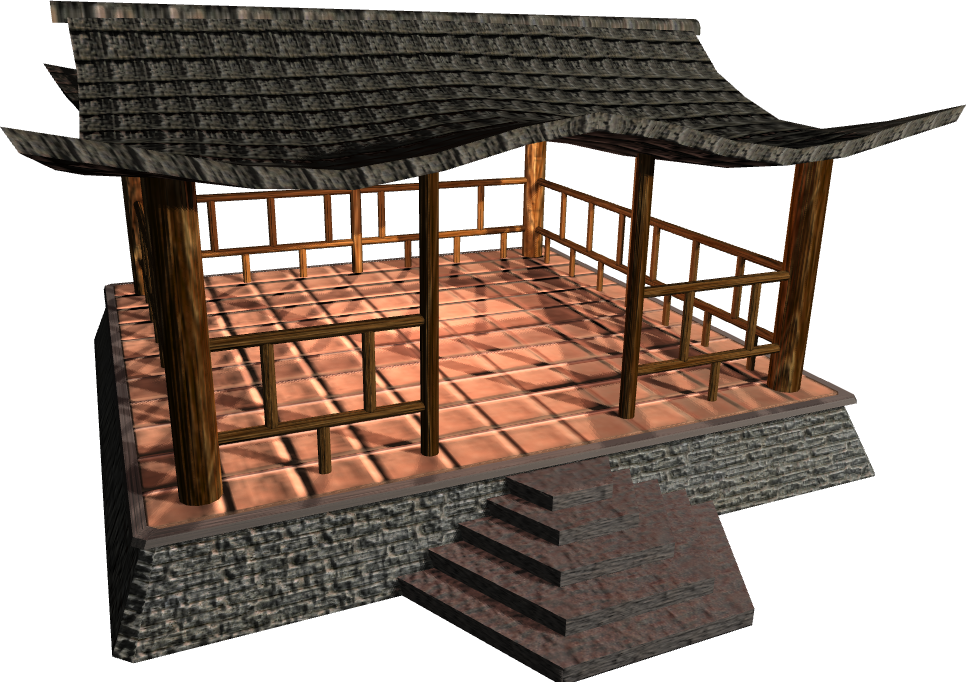
\includegraphics[width=2.19in]{rhan_shrine_5_everything}
  \caption{Bump mapping and 2 shadow maps on the same shape.}
}

\maketitle

\begin{abstract}
We demonstrate a flexible way to implement effects in X3D \cite{x3d:spec}
by shader programming.
Our approach allows to define the effects at appropriate places
(not only at Appearance, but also at particular light sources, texture and such).
It allows to seamlessly combine many effects, defined by X3D author,
with the shader defined internally by X3D browser.
Thus, it makes designing new effects in the GPU shading language trivial,
both for the browser implementors and for X3D authors. Various effects
cooperate automatically, and may be trivially composed by the X3D author.
And it still allows to design effects using the full power of GPU shading
language. We deliberately do not invent a new language, thus allowing
the authors the use all the shading language features for given GPU,
and allowing for easy implementation --- there is no need for any complex
language processing inside X3D browser.
\end{abstract}

\begin{CRcatlist}
  \CRcat{I.3.7}{Computer Graphics}{Three-Dimensional Graphics and Realism}{Color, shading, shadowing, and texture};
  \CRcat{I.3.6}{Computer Graphics}{Methodology and Techniques}{Languages, Standards}
\end{CRcatlist}

\keywordlist

\section{Introduction}

%% The ``\copyrightspace'' command must be the first command after the
%% start of the first section of the body of your paper. It ensures the
%% copyright space is left at the bottom of the first column on the first
%% page of your paper.
\copyrightspace

We present a technique for composing many shader snippets into a
single shader code. X3D browsers can use it to allow user and browser
shaders to coexist. Thus, users benefit from all the effects
implemented in the browser, even when they want to add some effect by
explicit shader code. Users can also seamlessly connect various
effects into a shape, without the need to adjust any shader source
code. Even the browser's implementation can be simplified, by using
the same mechanism to separate implementation of various effects
within a browser.

For an interesting example, consider three effects: shadows, bump
mapping, and lighting equations. Shadows provide an information that
either turns on or off a particular lighting contribution (or scales
this contribution, in case of soft shadows). Lighting equation
calculates light contribution, looking at material, light source and
normal at given geometry point. Bump mapping
\cite{vrmleng:bumpmapping} (in the simplest case)
modifies how the normal value is obtained: when bump mapping is used,
the normal is taken from the texture. So we have

$$ shadow(light) * light\_contribution(light, material, normal(point)) $$

In case of no shadows, shadow(x) = 1. In case of no bump mapping,
normal is determined by the geometry (per-face, or smoothed per-face),
and usually is passed as an already calculated attribute to the
shader.

We would like to be able to modify these three functions independently.
Independent effects may want to modify these functions, without knowing
about each other. Our goals are to:

\begin{enumerate}
\item Make shader programs much easier to create. That's because we
  can jump straight into the implementation of our imagined algorithm
  in the shader.
  We are only interested in modifying the relevant shader calculation
  parameter, and we can completely ignore other parts of the shader.

\item Make shader programs much more powerful. That's because our effect
  immediately cooperates with absolutely every normal feature of X3D rendering.
  This makes the implemented effect useful for a wide range of real uses,
  not only for a particular situation or a particular model (as it often happens
  with specialized shader code).
  All X3D light sources, textures, even other shader effects,
  are correctly applied.
\end{enumerate}

\section{Motivation and previous work}

Current shading description methods do not allow easy connecting
many effects into a single shader.

Shading source code files (GLSL, Cg) make no such way.

Effects formats (HLSL .fx, CgFX) allows to choose one technique, and
within it make passes. No way of automatically connecting one .fx file
with another.

One oldest solution: make a library of functions (like GLSL
functions), and allow to user to use them. But this is very bad and
limited. You cannot e.g. insert a shadow check right before adding the
light contribution (and still use browser code outside (to iterate
over lights) and inside (to calculate single light contribution)).

Another common solution is to arrange shaders in a pipe, where one
shader processes the result of another. This can be visualized as
layers of materials, where each layer modifies the previous
layer. However, this is again not flexible --- there's no way to plug
in your code in the middle of another shader's work.

An older solution, in the spirit of above, was also to perform
multi-pass rendering. However, this (in addition to lack of
flexibility of previous approach) makes also a loss of rendering
speed. In our work, we want to allow a single rendering pass to be as
powerful as it can.

%% (see also http://groups.google.com/group/blendertorenderman/browse_thread/thread/aaf07831b91be9db?pli=1 , confirms my findings)

Another approach is the Sh (ref:http://libsh.org/) language, which
allows writing shaders code (that can run on GPU) directly inside a
C++ program. For this, Sh extends the C++ language (through C++
operator overloading and macros tricks). It allows an excellent
integration between C++ code and shaders, hiding the ugly details of
passing variables between normal code (that executes on CPU) and
shader code (that usually executes on GPU). You can use
object-oriented methods there to create a general shader that can
later be extended through various means, like overriding virtual
methods. However, this is a solution closely coupled with C++. It's
suitable if you have a 3D engine in C++, and you want to use in your
own C++ program and extend it's shaders. In this paper, we want to
create a solution that is absolutely separate from the programming
language used to make a browser. Invoking a compiler to generate a
final GPU shader, not to mention teaching user's C++, is out of the
question.

%% ("Metaprogramming GPUs with Sh", http://books.google.com/books?id=8RX4RmFRLmgC&pg=PA79&lpg=PA79&dq=ShAttrib2f&source=bl&ots=IOxd1-BQLL&sig=AIPgFRmbodNpCLWmwk-QV5JUjVo&hl=pl&ei=EylRTe7RB8qeOsiQ1aQI&sa=X&oi=book_result&ct=result&resnum=7&ved=0CEkQ6AEwBg#v=onepage&q=ShAttrib2f&f=false )

At the end, we would like to mention a solution from a completely
different domain, that is surprisingly similar to ours in some ways.
Drupal, an open-source CMS system written in PHP,
has a very nice system of modules. Each module
can extend the functionality of the base system (or other module)
by implementing a \textit{hook}, which is just a normal PHP function
with a special name and appropriate set of parameters. Modules can also define
their own hooks (for use by other modules) and invoke them when appropriate.
This creates a system where it's trivially easy to define a hook,
and to use a hook.
Many modules can implement the same hook and cooperate without any problems.
The whole hook system is defined completely in PHP, as it's a scripting
language, and you can query the list of loaded functions by name,
and call function by name.

This is actually quite similar to our base idea of combining effects
inside Appearance.effects field. Our effects are similar to
Drupal's modules, as our ,,plugging points'' are analogous to Drupal hooks.
Our effects can define functions with special names to override
standard shader behavior. They can also define new names of plugs, for other
effects to use. Of course we also have some special problems
(shading language is quite far from a scripting language,
so defining hooks is done by smart textual replacements)
and some special opportunities (we can define effects at
the appropriate nodes of X3D, like textures and lights sources,
as we don't want to throw all the effects in one bag).

\begin{figure*}[t]
  \centering
  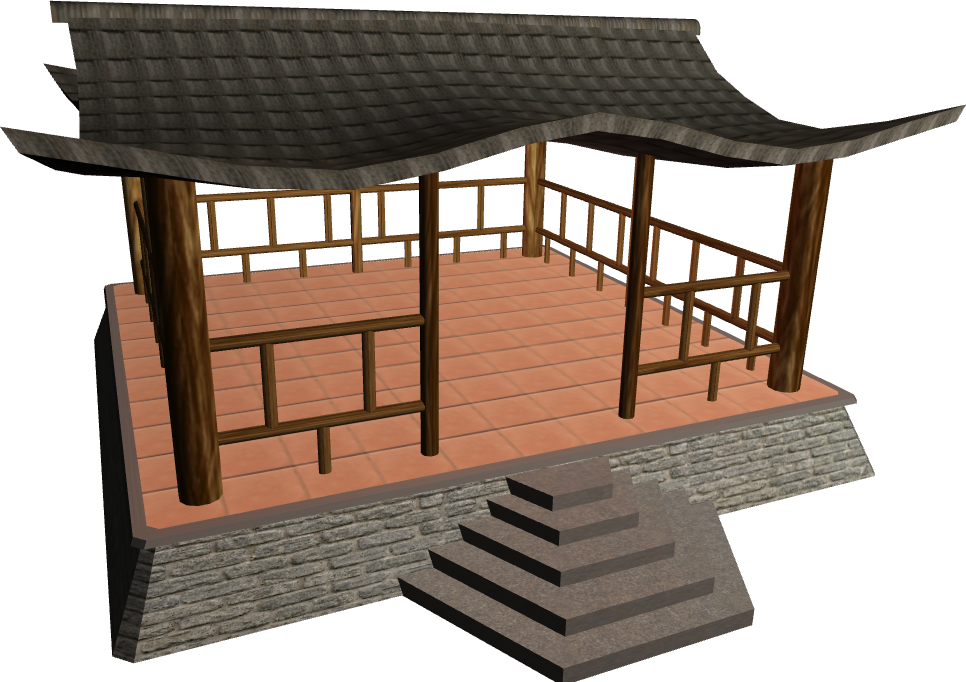
\includegraphics[width=2.3in]{rhan_shrine_0}
  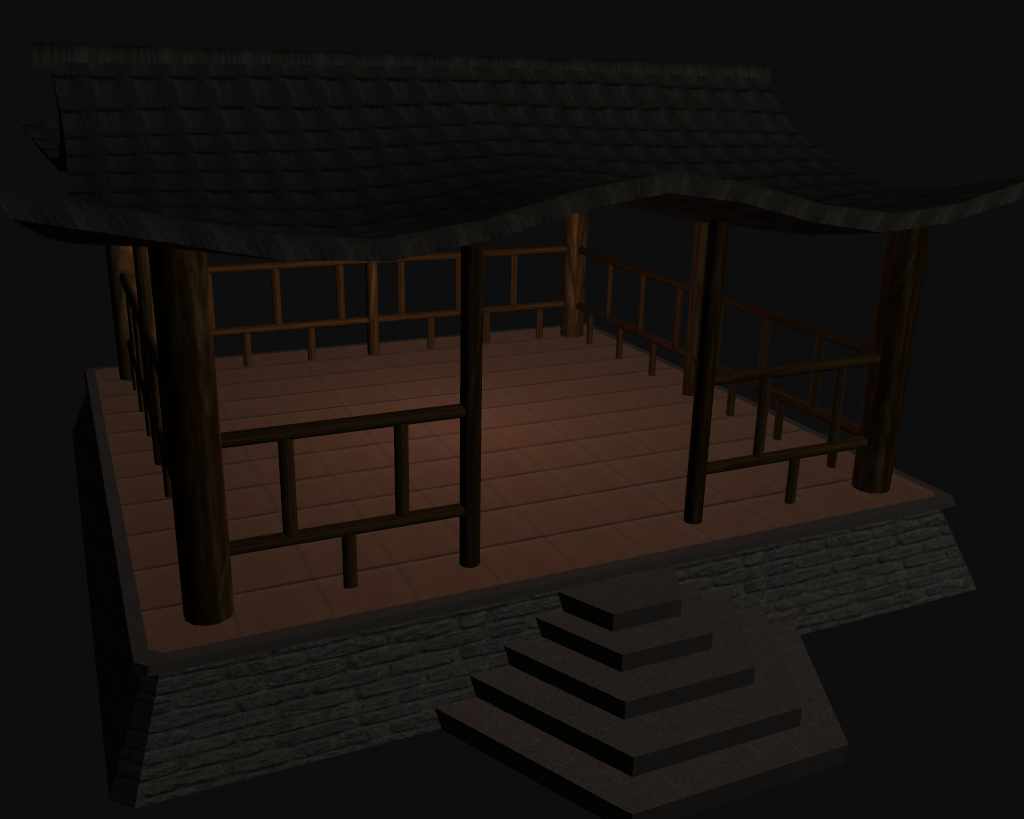
\includegraphics[width=2.3in]{rhan_shrine_1_per_pixel_lighting}
  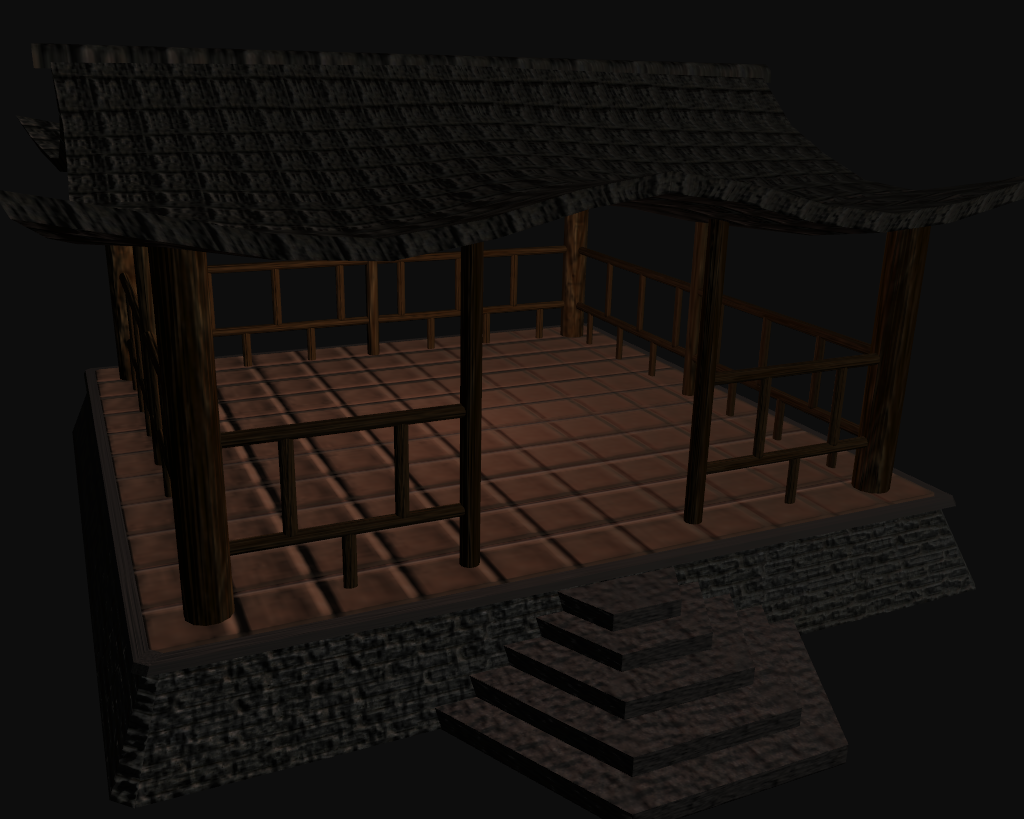
\includegraphics[width=2.3in]{rhan_shrine_2_bump_mapping}
  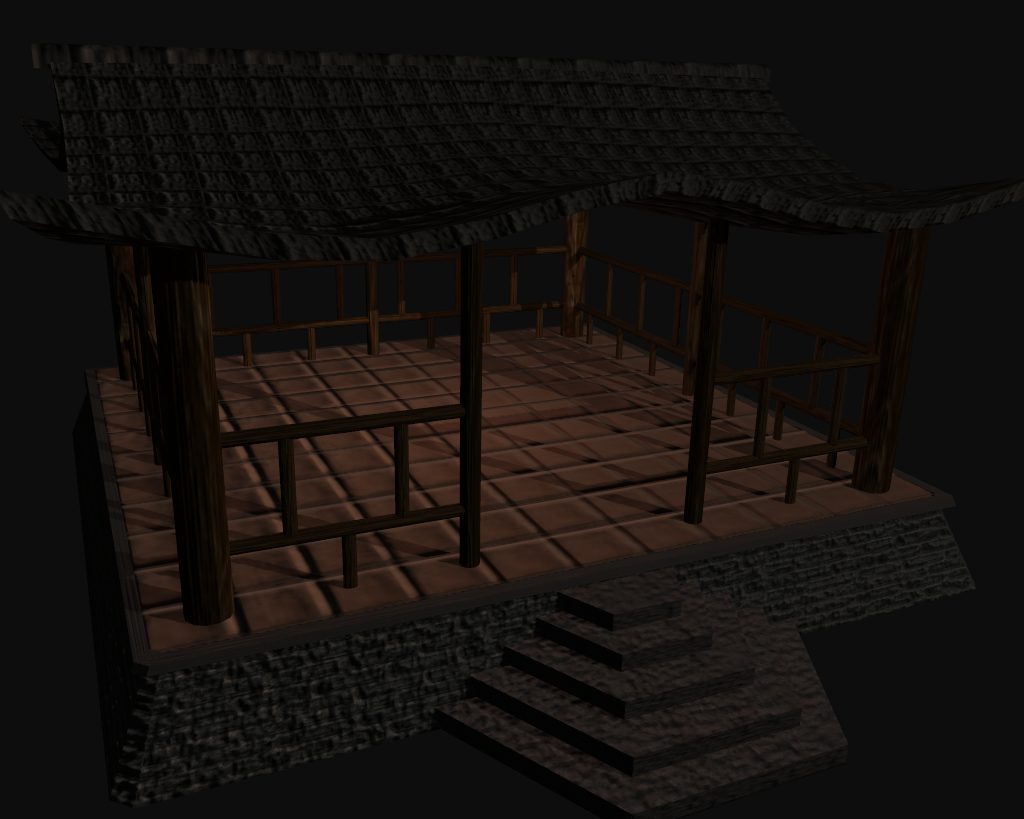
\includegraphics[width=2.3in]{rhan_shrine_3_shadow_1st}
  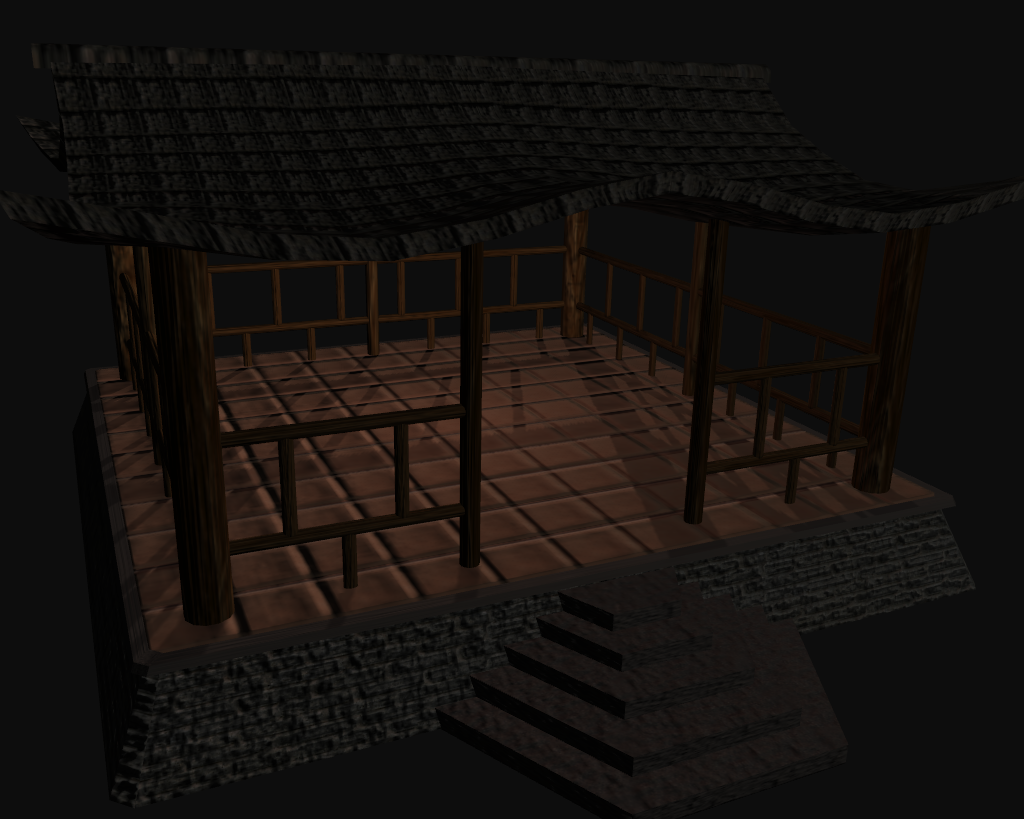
\includegraphics[width=2.3in]{rhan_shrine_4_shadow_2nd}
  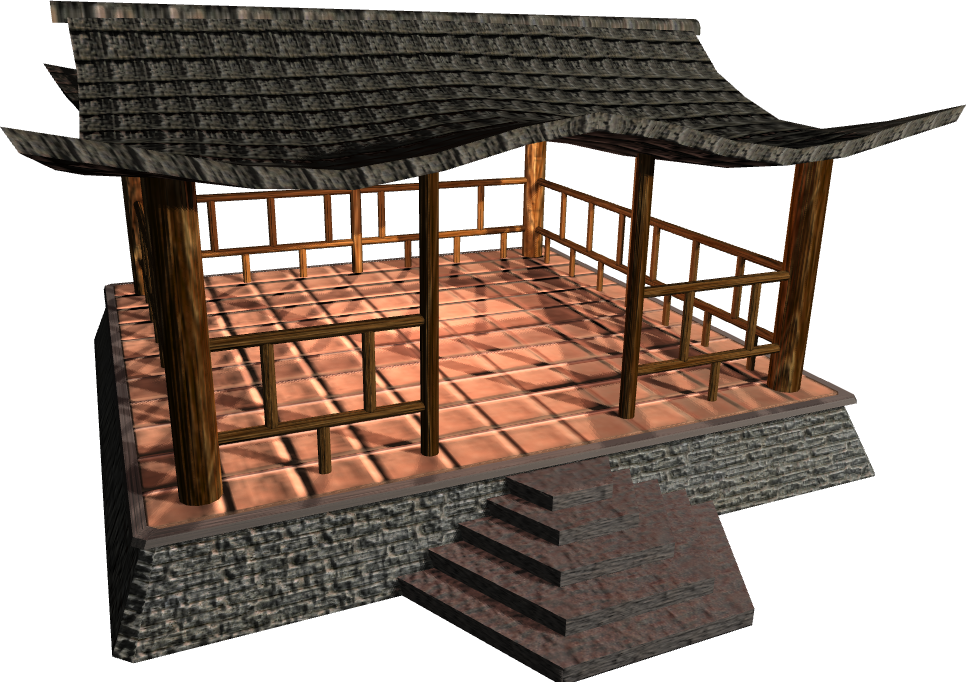
\includegraphics[width=2.3in]{rhan_shrine_5_everything}
  \caption{Japanese shrine model with more and more effects applied: Gouraud shading,
Phong shading (per-pixel lighting), bump mapping, shadows from 1st light,
shadows from 2nd light, shadows from both lights.}
%%  \label{fig_xxx}
\end{figure*}

\section{Plugging}

The basic idea of our approach is that a shader source code defines
a points when a calls to user-defined functions may be inserted. The mechanism
allows very easily to define new plugging points, and to use
them. Moreover, user shaders and browser internal shaders have the
same means to define and use plug points. This allows to connect
shaders (both user and browser) in a variety of ways.

A trivial example of an effect that makes colors two times brighter
follows. This is written in X3D classic encoding,
you should add this inside any \texttt{Appearance} node:

\begin{Verbatim}[commandchars=\\\{\},frame=single]
effects Effect \{
  language "GLSL"
  parts EffectPart \{
    type "FRAGMENT"
    url "data:text/plain,

\textbf{    void PLUG_texture_apply(}
\textbf{      inout vec4 fragment_color,}
\textbf{      const in vec3 normal)}
\textbf{    \{}
\textbf{      fragment_color.rgb *= 2.0;}
\textbf{    \}}"
  \}
\}
\end{Verbatim}

It defines a GLSL function named \texttt{PLUG\_texture\_apply}
within an \texttt{EffectPart} node. Function names starting with \texttt{PLUG\_}
are special, they enhance some standard shader calculation. In particular
the \texttt{PLUG\_texture\_apply} is used after the normal texture colors are applied,
but before the alpha test, and is a usual place to ,,just modify the pixel color''.
\texttt{fragment\_color} is an \texttt{inout} parameter, by modifying it
you modify the color that will be displayed on screen (and the alpha that will
be tested).

We have a short reference (at the end of this document) of all
the plugging points available in our shaders. For each plugging point,
like this \texttt{PLUG\_texture\_apply}, we define a list of it's parameters
(you have to declare them exactly the same in your code), and we define
when it is called.

Various ways of defining and using ,,plugging points'' (which we'll just call
,,plugs'' from now on) are possible:

\begin{myenumerate}
\itemsep 0pt
\item Browser shaders can be connected with each other. For example, we
have a basic shader code that defines lighting and texturing. Our bump
mapping is implemented by simply plugging the code in the appropriate
places in this base shader. This way, the base shader is completely
independent from the bump mapping implementation. We can switch bump
mapping implementations (for example, use bump texture from image or
some random noise) without trouble.

So even inside the engine, this allows for much easier shader generator.

\item User shaders may plug into browser shaders. This is the most usual
case. Our shaders define various points when you can plug your code,
and override or enhance our shading.

\item User shaders may also plug into another user shaders. User shaders
can trivially (by just adding a "magic" comment) define new plugging
points, which are usable by other user shaders. User effects can
define plugging points, which are available to the following effects
on the Appearance.effects list.

\end{myenumerate}

We allow user shaders (defined in the \texttt{ComposedShader} and such nodes) to
define additional plugging points. User shaders can use our plug names
(and thus work with the same effects), or they can invent their
own. They can also always add new plug points.

When you don't use an explicit shader (like \texttt{ComposedShader} node),
browser uses it's own internal basic shader. This shader is then
extended by effects like bump mapping (coming from internal browser
implementation), or by user effects. But you can also define your own
\texttt{ComposedShader} node. Then your own shader is enhanced by the
browser. If you define the same (or compatible) plugging
points, then the browser effects will be even added to your own
shader. And of course user effects are added to your shader.

In summary, the system works regardless if you use or not an explicit
shader on \texttt{Appearance.shaders} list.

\subsection{Effect node}

In the X3D file we add a field

\begin{mycode}
\underline{Appearance}
\begin{Verbatim}[commandchars=\\\{\}]
MFNode [] \codeem{effects} [] # Effect
\end{Verbatim}
\end{mycode}

that can hold any number of

\begin{mycode}
\underline{Effect : X3DChildNode}
\begin{Verbatim}[commandchars=\\\{\}]
SFString [] \codeem{language} ""
  # Just like ComposedShader.language.
  # This effect will be used only when
  # the base shader (browser internal
  # or selected from Appearance.shaders)
  # has the same language.
SFBool [in,out] \codeem{enabled} TRUE
  # Allows to easily turn on/off the effect.
  # You could also remove/add the node
  # from the scene, but often toggling
  # this field is easier for scripts.
MFNode [] \codeem{parts} [] # EffectPart
  ... additionally you can
      declare new fields and events,
      that will be passed
      as uniform values to the shader,
      just like for ComposedShader node ...
\end{Verbatim}
\end{mycode}

\begin{mycode}
\underline{EffectPart : X3DNode, X3DUrlObject}
\begin{Verbatim}[commandchars=\\\{\}]
SFString [] \codeem{type} "VERTEX"
  # Just like ShaderPart.type,
  # allowed values are
  # FRAGMENT | VERTEX |
  # (once supported) GEOMETRY.
MFString [] \codeem{url} []
  # Source code, just like ShaderPart.url.
  # May come from an external file (url),
  # or inline (following "data:text/plain,").
  # In XML encoding, may also be inline
  # in CDATA.
\end{Verbatim}
\end{mycode}

The functions you want to override are automatically detected by names
starting like \texttt{PLUG\_}.

In a single \texttt{EffectPart} node, you can define many \texttt{PLUG\_}
functions. However, you can only plug functions into the declared shader
type. For example, you cannot plug into \texttt{texture\_apply} when
your type is \texttt{VERTEX}.
If your effect requires some processing per-vertex and some per-fragment,
you will probably use two \texttt{EffectPart} nodes, with appropriate types.
While this may seem like an arbitrary limitation,
this reflects how shader parts are declared in shading languages with
separate namespaces for vertex and fragment parts (like GLSL).
A single part may declare variables (uniform, varying and such),
and many functions that use them. But it must be completely within
one shader type.

At one point we tried the approach
to not look at any special function names in GLSL code,
and instead define a plug name in the separate field of the \texttt{EffectPart}
node. However this produced ugly code --- you had to split your algorithm
into many \texttt{EffectPart} nodes, each often containing only 1 or 2 lines
of code. Especially bad was the fact that you had to declare uniform variables
in a separate effect part, which in turn means that we cannot place
your effects parts in separate namespaces (like a compilation unit in GLSL),
which in turn makes the usage less secure.
Detecting \texttt{PLUG\_} function names in GLSL code is very easy,
and turned out to be the cleaner solution.

In case of shading languages that have separate compilation units
(like OpenGL shading language) the implementation may choose to place
each effect part in such separate unit. This allows for cleaner error detection
(as the parsing errors in effect code will not cause errors elsewhere,
and error messages will refer to line numbers in actual user code).
This also allows some namespace separation. For example, uniforms defined in one
effect part may not be visible in the other part, as they should be placed
in a separate namespace (like a separate compilation unit for GLSL) if possible.

All the effects on this list (with suitable language, and with
plugging points defined by the browser shader, or active shader on
\texttt{Appearance.shaders} list) will be used. Note that this is contrary to
the \texttt{Appearance.shaders}, which chooses only one shader.
For effects, we choose all of them (that are suitable).

\needspace{1in}
The most basic idea of this paper is to allow one to define two
independent shader effects, and then seamlessly connect them by simply
placing them both on \texttt{Appearance.effects} list. This also allows to
define a library of effects, that can be composited without any work
needed by user.

\begin{figure}[H]
  \centering
  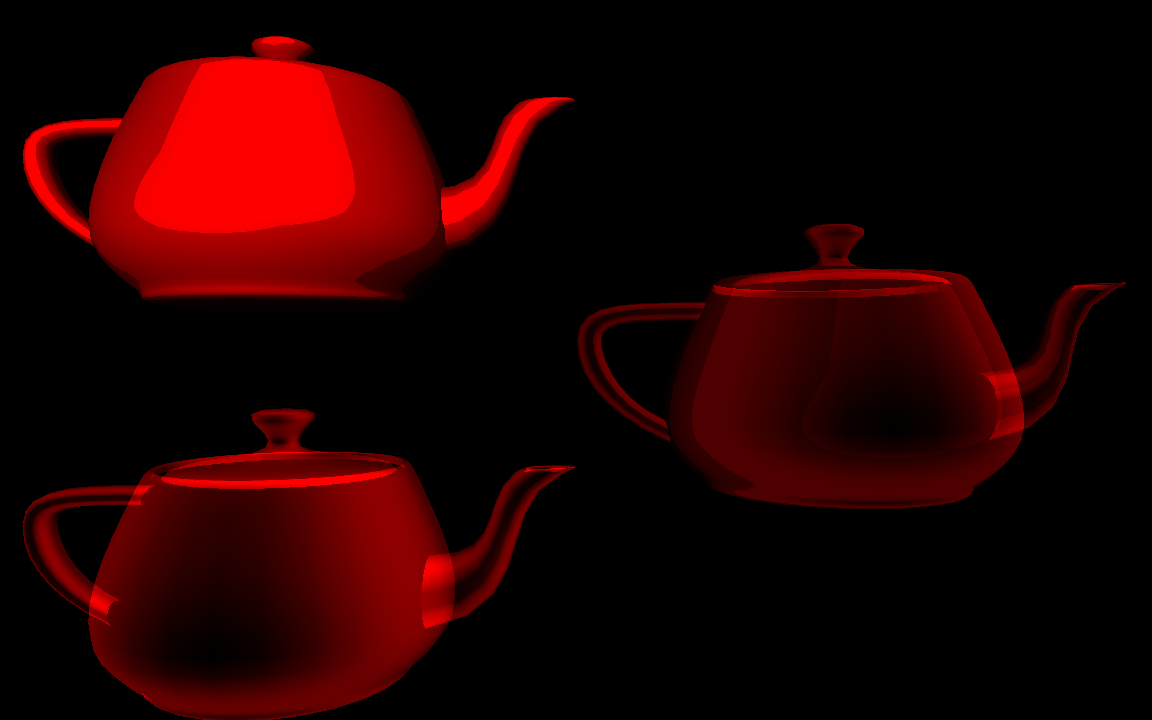
\includegraphics[width=3in]{fresnel_and_toon}
  \caption{Toon and Fresnel effects combined.}
\end{figure}

Note that all our nodes benefit from X3D mechanism to reuse the nodes
by reference (the DEF / USE keywords). Reusing the \texttt{Effect} nodes
is most natural, and allows to combine existing effects in any desired way.
Reusing the \texttt{EffectPart} nodes is also useful, when some effects
would like to share a particular piece of code. For example,
you can create an \texttt{EffectPart} with a library of useful
shading language functions, and reuse if for various effects.

\subsection{Effects for a group of nodes}

Our \texttt{Effect} node is a descendant of \texttt{X3DChildNode},
and can be placed directly within X3D grouping nodes like
\texttt{Group} and \texttt{Transform}, and at the top level of the X3D file.
Such effect will apply to all the shapes within given grouping node.
The scope rules follow the X3D conventions for other nodes,
like pointing device sensor nodes and \texttt{LocalFog}.

The \texttt{LocalFog} is especially worth mentioning. Using this mechanism,
a browser can implement the \texttt{LocalFog} node as a prototype
that expands to our \texttt{Effect} node. This gives you a 100\% correct
implementation of the standard \texttt{LocalFog} node, as is trivially easy.

As one of the demos, we have implemented a realistic
animated volumetric fog, where the fog density is stored in
a 3D smooth noise texture (idea from \cite{humus:volumetricfog}).
In a fragment shader, the 3D texture is sampled
along the line between the camera and pixel position. This makes a very
convincing effect of a dense fog. Since it is implemented as an effect,
it can be instantly used with various lighting and texturing conditions
--- it simply works for all X3D shapes.

\begin{figure*}[t]
  \centering
  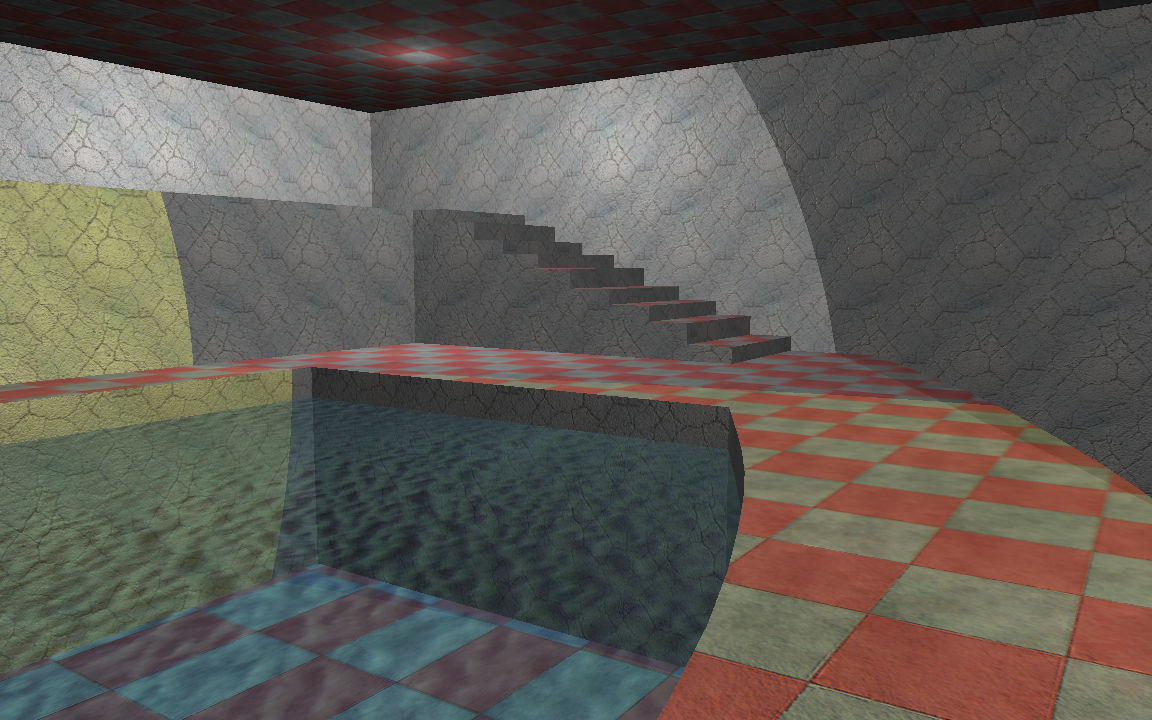
\includegraphics[width=2.3in]{volumetric_animated_fog_no_fog}
  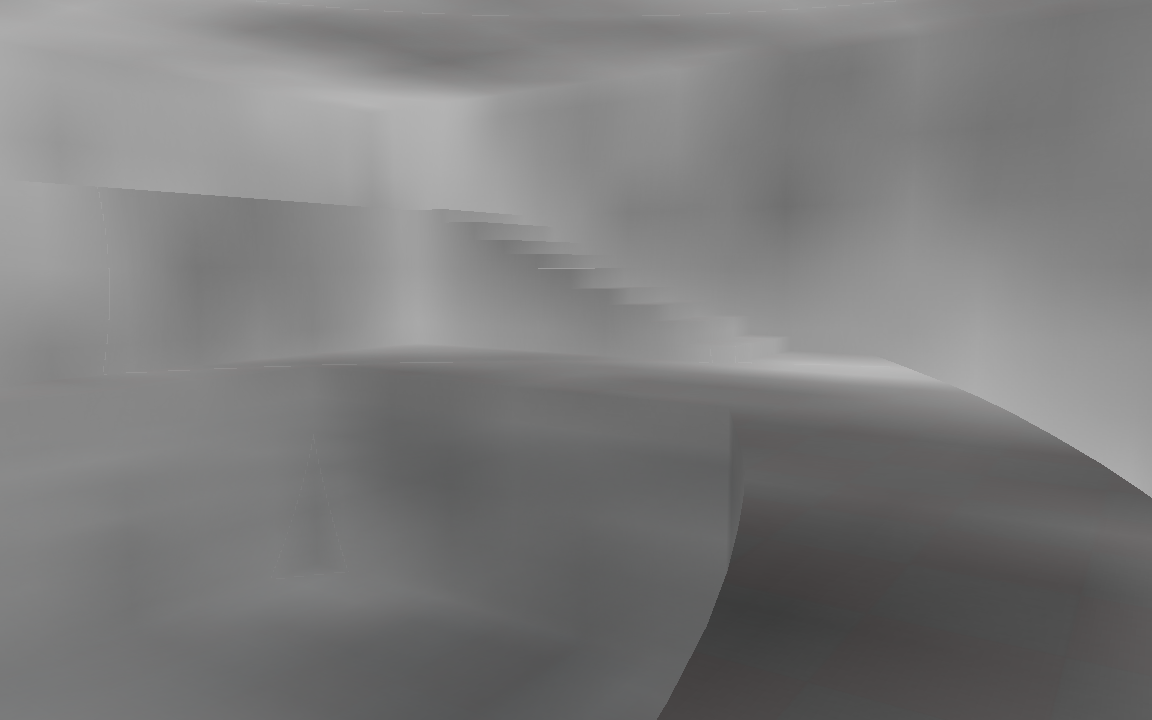
\includegraphics[width=2.3in]{volumetric_animated_fog_no_light}
  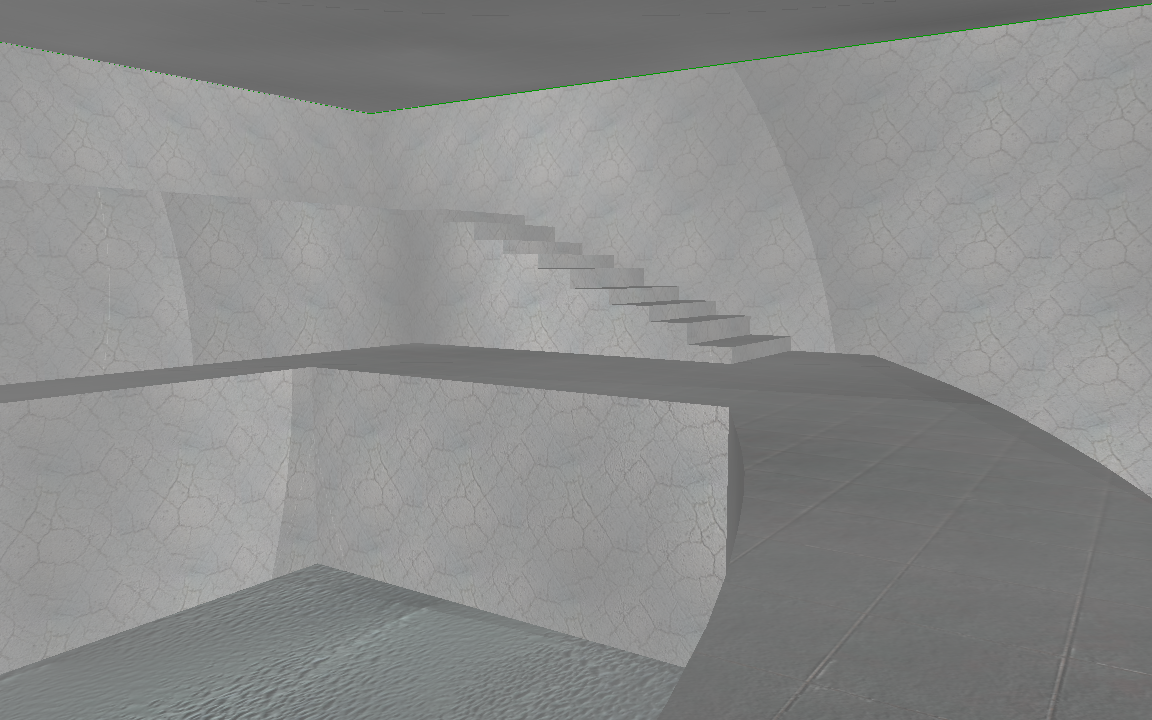
\includegraphics[width=2.3in]{volumetric_animated_fog_all}
  \caption{Volumetric fog scene: 1) No fog; 2) No lighting; 3) Lights and fog.
Note that the fog is assumed to have it's own ambient lighting,
so it colors the image even in the 2) case.}
\end{figure*}

\subsection{Light sources effects}

The real power of our system comes from the fact that some nodes,
like light sources and textures, can define their own effects.
So you can easily define a shader specific for a given light source,
or texture.

We add the \texttt{effects} field for every light node:

\begin{mycode}
\underline{X3DLightNode}
\begin{Verbatim}[commandchars=\\\{\}]
MFNode [] \codeem{effects} [] # Effect
\end{Verbatim}
\end{mycode}

You can modify the light source contribution, or even replace the default
calculation of light source contribution. In the second case,
the default calculation will not even be used in the shader,
so it will not slow down the calculation without a reason.

\subsection{Texture effects}

Just like the light sources, also each texture node may define it's own effects:

\begin{mycode}
\underline{X3DTextureNode}
\begin{Verbatim}[commandchars=\\\{\}]
MFNode [] \codeem{effects} [] # Effect
\end{Verbatim}
\end{mycode}

You can use the \texttt{effects} field
inside any \texttt{X3DTextureNode} to enhance and modify the look of any
standard texture node, like \texttt{ImageTexture}.
You can use a plug \texttt{texture\_color},
that allows you to modify the texture color, knowing the current texture
coordinates and such.

\subsubsection{ShaderTexture effects}

We introduce a new X3D node designed specifically for generating
textures using the shading language. This is especially suitable
if your texture is defined completely by the shaders.
The texture contents are not stored anywhere (not even on GPU),
the X3D browser doesn't manage any texture resources and such.
From a GPU point of view, there is no texture\footnote{But the spoon is real,
we swear.}. There is only a shader function that generates colors
based on some vectors.

While not strictly necessary, it's comfortable to wrap a texture generation
function inside the \texttt{ShaderTexture} node, that is treated much
like other X3D texture nodes. This allows the authors to provide texture
coordinates (explicit or generated) for this texture, using all the standard
tools available in X3D.

The new texture node specification:

\begin{mycode}
\underline{ShaderTexture : X3DTextureNode}
\begin{Verbatim}[commandchars=\\\{\}]
MFNode [] \codeem{effects} [] # Effect
SFString [] \codeem{defaultTexCoord} "BOUNDS2D"
  # ["BOUNDS2D"|"BOUNDS3D"]
\end{Verbatim}
\end{mycode}

Actually, the \texttt{effects} field is already defined at
the \texttt{X3DTextureNode} class (see above).

You should include an effect overriding at least the \texttt{texture\_color}
plug, otherwise texture contents are undefined. Our implementation actually
sets the default texture color to pink (RGB(1, 0, 1)), so it stands out,
reminding you to override it.

The \texttt{defaultTexCoord} says what texture coordinates to generate,
if the geometry doesn't specify any texture generation method.

\begin{myenumerate}

\item
  \texttt{"BOUNDS2D"} means that the algorithm described in the specification
  for {IndexedFaceSet} should be used. This adapts 2D texture coordinates
  to two largest bounding box sizes.
  It's most suitable for 2D textures that use only 2D coordinates
  (ignoring other coordinates, or assuming they are always 0, 1).

\item
  \texttt{"BOUNDS3D"} means that the algorithm described in the specification
  of \textit{Texturing3D} component (section \textit{"Texture coordinate generation for primitive objects"}).
  This adapts 3D texture coordinates to bounding box sizes.
  Most suitable for 3D textures (you can ignore the 4th texture coordinate
  component, or treat it as homogeneous, as \texttt{"BOUNDS3D"} will always
  set it to 1).

\end{myenumerate}

Remember that the texture coordinates can be always explicitly specified
at the geometry, by explicitly listing the coordinates (nodes
\texttt{TextureCoordinate}, \texttt{TextureCoordinate3D},
\texttt{TextureCoordinate4D}) or by explicitly giving the generation
algorithm (nodes \texttt{TextureCoordinateGenerator},
\texttt{ProjectedTextureCoordinate} \footnote{
    Note that our implementation has some extensions
    to \texttt{TextureCoordinateGenerator}. In particular
    \texttt{"BOUNDS2D"} and \texttt{"BOUNDS3D"} are also valid names for
    \texttt{TextureCoordinateGenerator.mode}, see
    \cite{vrmleng:texcoordbounds}.
    Projective texture mapping by \texttt{ProjectedTextureCoordinate}
    is also our extension, see \cite{vrmleng:projectivetexturing}.}).
The \texttt{defaultTexCoord} says only what is the default approach,
when you don't use \texttt{texCoord} at the geometry node.
The idea is that using a \texttt{ShaderTexture} should be as comfortable
as any other normal texture.

\subsubsection{When to use ShaderTexture}

For textures that are not \texttt{ShaderTexture},
when the \texttt{texture\_color} plugs are called,
the internal shaders already calculated the initial texture
color by actually sampling the texture image. This is useful for you if you
want to modify this color. If you simply want to ignore the normal
texture color, and always override it with your own, consider using
the special \texttt{ShaderTexture} node instead. Using
a normal texture node (like \texttt{ImageTexture}) for this
would be uncomfortable, as you would have to load a dummy texture image,
and the shaders could (depending on optimization) waste some time
on sampling a dummy texture color that will be actually overridden later.

Remember that in all cases (effects at \texttt{ImageTexture},
at \texttt{ShaderTexture}, etc.) you can always use additional
textures inside the effect. Just like inside a standard \texttt{ComposedShader},
you can declare an \texttt{SFNode} field inside an \texttt{Effect}
to pass any texture node to the shader as uniform value.
This allows you to base your effects calculation on any number of textures,
and combine them in any way you like. The only difference
between various \texttt{X3DTextureNode} descendants is what the browser
does automatically for you, that is what color is passed
to the first \texttt{texture\_color} plug.

\begin{figure}[H]
  \centering
  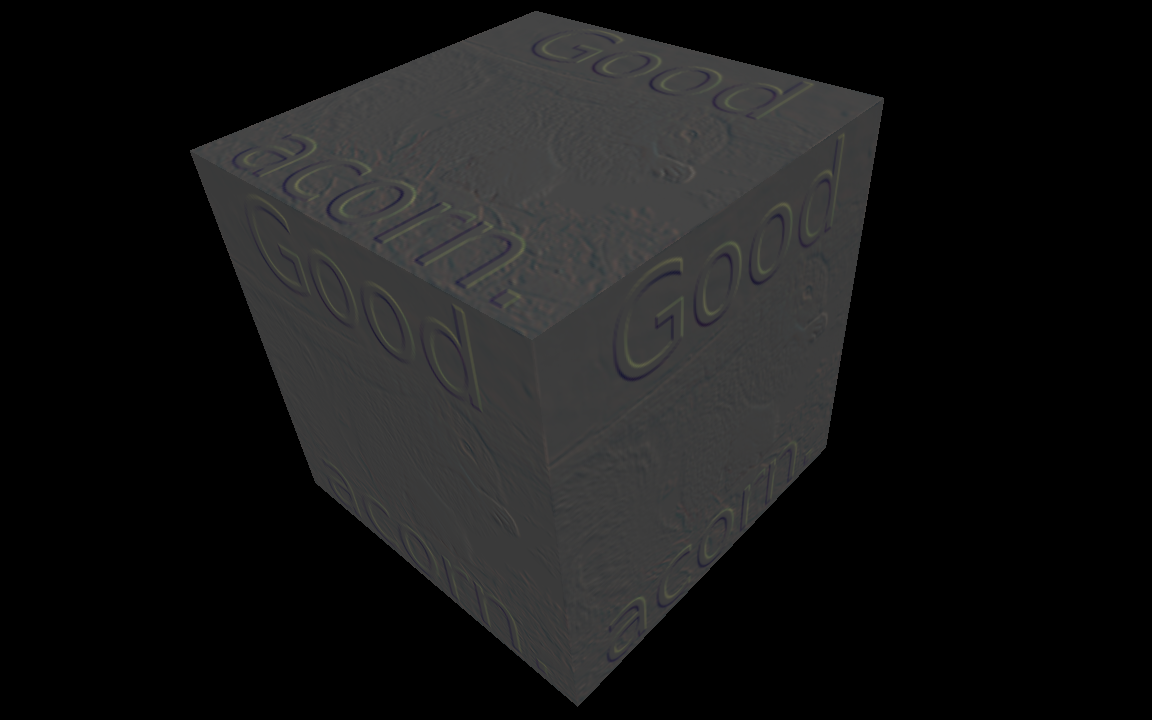
\includegraphics[width=3in]{shader_texture_edge_detection}
  \caption{ShaderTexture showing an edge detection operation on normal ImageTexture.}
\end{figure}

\subsubsection{No aliasing}

The nice thing about the effects used on textures (both for \texttt{ShaderTexture}
and for standard texture nodes) is that they are sampled at each
screen fragment. So your effects are not concerned with texture filtering
options. You just use the texture coordinate, passed for example to the
\texttt{texture\_color} plug.

\begin{figure}[H]
  \centering
  
\includegraphics[width=3in]{shader_texture_no_filtering_problems}
  \caption{Yellowish arc is done by a texture effect, as so is not
    affected by the pixelated look of the base image texture.}
\end{figure}

\section{Defining your own plug points}

When you write shader code, you can define your own plug points by a
magic comment:

\begin{mycode}
/* PLUG: plug-name (param1, param2, ...) */
\end{mycode}

This defines a point when multiple user plugs may be added. Each
Effect with name matching given plug-name will cause a
definition of a new function, that will be called with given parameters
at this place.

This is often useful for processing some parameter
repeatedly (like adding or modulating the fragment color),
so one or more of the parameters are usually allowed to be processed
as \texttt{inout} parameters.

Multiple code pieces may be added to the given plug point.
So multiple effects may use the same plug point. They are added
in the order they are specified in the Appearance.effects list
(although, preferably, for most effects this order will not matter).

Moreover, the same plug may be declared many times in the source shader.
This means that a single \texttt{PLUG\_xxx} function will be called
many times. This is typically useful when your shader calculation is naturally
expressed as a loop, but you had to unroll this loop for shader source
(for example, to slightly tweak some loop iterations).
The plug names that are available per-light source and per-texture
are an example of this. If you use the \texttt{PLUG\_texture\_color}
inside \texttt{Appearance.effects}, you can change the color of all
the textures (even shader textures).
Similarly, if you use the \texttt{PLUG\_light\_scale}
inside \texttt{Appearance.effects}, you can change the intensity
of all the light sources on the given shape.

Currently all the plugs must be procedures, that is their result type
must be declared as \texttt{void}. We have been considering
a possibility of functions, where part of the calculation may be replaced
by a function call to a plug function. While not difficult to implement,
this idea seems like a useless complication after many tests.
Procedural plugs are easier to declare, as the call to the plug
may be simply inserted, while in case of function it will have to replace
some previous code. This also means that using a procedural plug
\textit{never} replaces or removes some existing code, which is a very nice
concept to keep. We want the effects to cooperate with each other,
not to ,,hijack'' from each other some parts of functionality.

\subsection{Where the forward declarations are placed}

Special comment \texttt{/* PLUG-DECLARATIONS */} may be used
near the beginning of your shader source code. It is only useful
if your shader code defines any new plugging points, that is if you
have any magic \texttt{/* PLUG: ... */} comments inside.
When some other effect uses your plugging point, the browser adds
an appropriate call to a function in that effect.
Additionally, the browser has to declare the function,
because it may be in a separate compilation unit (in case of GLSL),
or just defined later in the code.
These (forward or external) declarations are inserted at
the point of special \texttt{/* PLUG-DECLARATIONS */}
comment, or (when it is missing) simply at the beginning of your shader source.
This applies in the same way to shader code inside an \texttt{EffectPart},
or inside standard X3D node like \texttt{ShaderPart}.

Using \texttt{/* PLUG-DECLARATIONS */} may be necessary
as some shading language directives are required to be placed before
all normal declarations. For example, in case of OpenGL shading language,
the \texttt{\#version} as well as some \texttt{\#extension} directives
must occur at the beginning of the shader code. You should place
\texttt{/* PLUG-DECLARATIONS */} after such directives,
and before any \texttt{/* PLUG: ... */} declarations.

\subsection{Why plugs are defined as comments}

The nice feature of our magic /* PLUG ... */ comments is that a shader source
is still valid even if you completely ignore the plugs. For example,
you can write your custom ComposedShader node, defining some plugs,
and for browsers that understand them --- the plugs can be used,
for other browsers --- plugs will be gracefully ignored (but still
the shader will run, although without any effects).

\subsection{Plugs from effects}

You can define plug points both inside your custom ComposedShader code,
as in the ,,effects'' code. In the latter case, the plug points
are only available for the following effects of the same node.

\subsection{Invalid shader code}

We guarantee the behavior only if the provided shading language code
is a correct, self-contained code.
X3D browser doesn't validate code in any way, so any error (like undeclared
variable, like unterminated block (,,{'' without matching ,,}''),
like unterminated comment) may be only detected after the complete shader
is determined and compiled by the GPU.

Although in case of shading languages with separate compilation units,
the separation is actually better, and parsing errors will cause
problems in your own code only. Still, by writing incorrect code,
you can cause the whole shader to malfunction.

In all our practical cases, this didn't cause any problems.
Since you code each effect separately, you also test them separately,
and in practice it's usually obvious what problem causes the parsing error.
This is also a direct consequence of our decision to \textbf{never require
the browser to parse the shader code}.

It should be noted however that in particularly nasty cases,
a deliberately poorly coded effect may cause troubles for other effects.
In particular, since you can use \#define and macros in your effect code,
you can do nasty tricks to break other effects. You can make them compile,
but function incorrectly. However, we don't consider
it a real problem. You really have to deliberately want to do something bad,
and often use an internal knowledge, to achieve something bad.
It doesn't happen by accident in our experience.
%% And you may need to use the internal knowledge
%% how the other effects are implemented (maybe how they are implemented
%% inside the browser).

Note that this isn't a security problem --- bad shader code only breaks
rendering of a particular shape. And X3D ComposedShader node allows users
to execute any shading language code anyway. So if there's anything dangerous,
you could do it without using our effects framework anyway.

\section{Usage examples}

Remember that effects may define their own uniform variables,
just like normal shader node. So you can pass your own textures
to effects. For example you can write an effect that mixes a couple of textures,
using any information available in the shader as a criteria for mixing.
You can also pass any other values for an effect, for example you can
pass the current time from a \texttt{TimeSensor} and make dynamic effects.

\begin{figure}[H]
  \centering
  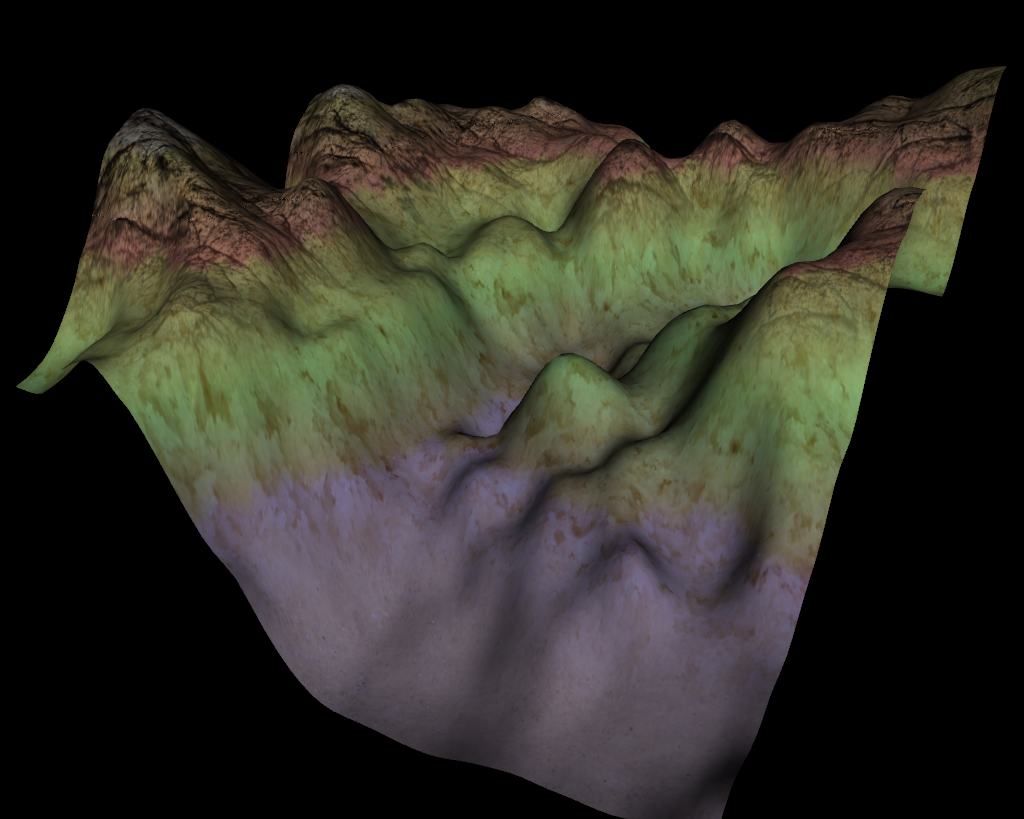
\includegraphics[width=3in]{terrain}
  \caption{ElevationGrid with 3 textures mixed based on height by GLSL effect.}
\end{figure}

An example effect for a light source is to use a fancy shape and equation
for light's spot.

\begin{figure}[H]
  \centering
  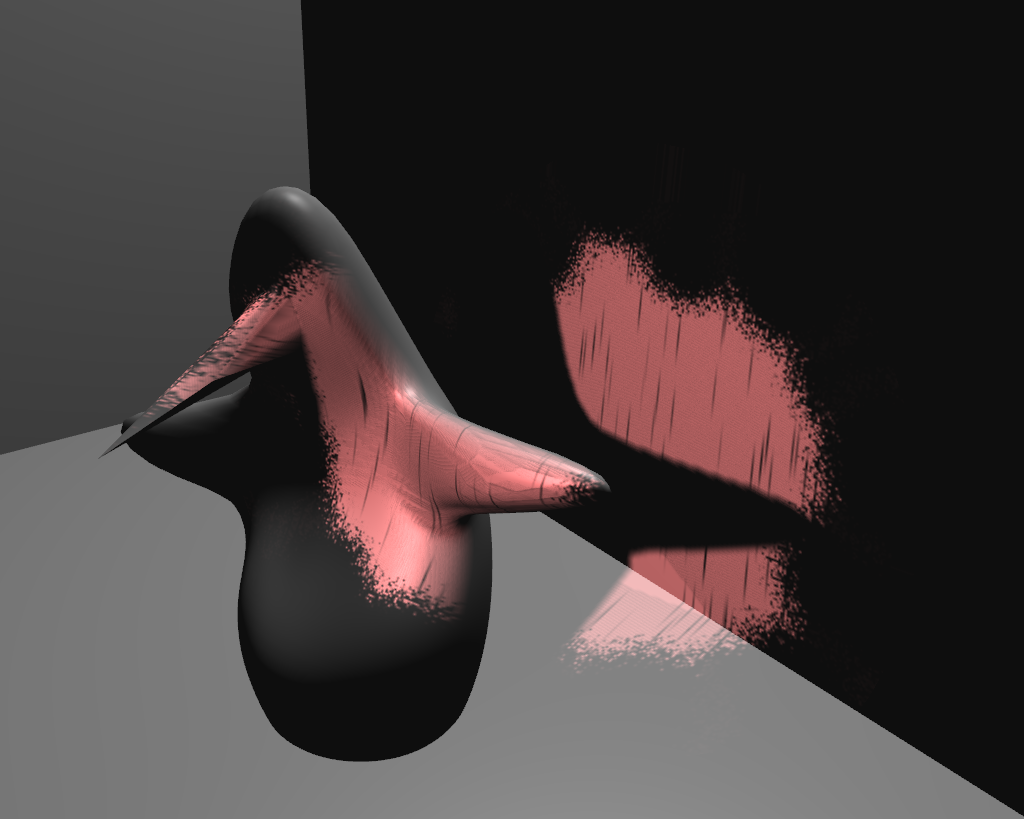
\includegraphics[width=3in]{fancy_light_spot_shape}
  \caption{Textured spot light with shadow.}
\end{figure}

Even inside the browse implementation, using plugs to implement internal
effects allows for a great code simplification and separation.
Our bump mapping effect is done purely by using plugs.
So it has a clean and short implementation. It also shows that
X3D authors could implement perfect bump mapping themselves,
without any traditional hassles. For example, bump mapping can be
achieved using standard \texttt{ComposedShader} as well,
but then you have to write all this ,,boilerplate'' code to also deal
with all the possible lighting and textures configurations.
Well, the browser is still useful to calculate nice tangent vectors,
although an authoring program could generate GLSL attributes for them as well.

Same thing with shadow maps, they only plug to the \texttt{light\_scale}
calculation of appropriate light.

Water is very nice to implement by our effects, as a proper water simulation
is naturally a combination of a couple effects.
You want to simulate waves, so you want to vary vertex
heights or vary normals per-fragment (for best results, a mixture of both).
You also want to simulate the fact that water has reflections, and
is transparent. We have implemented a nice water using this approach,
with two independent effects.

Our approach also allowed us to easily implement and test
two alternative versions for generating water normals.
One approach was to take normals from the pre-recorded sequence of images
(encoded inside \texttt{MovieTexture},
with noise images generated by Blender renderer).
The second approach was to calculate them on the fly from
a generated smooth 3D noise. We could immediately test our alternative versions
of the ,,water normal effect'' with the same, unmodified,
,,water reflection / refraction effect''.
(As for the results about which one is better: predictably, we showed
that using GPU noise is slower, requires a better GPU,
but also improves the quality noticeably. With GPU noise, there is no problem
with aliasing of the noise texture, and the noise parameters can be adjusted
in real-time.)

Our effects idea allowed us also to implement the two alternative versions
of ,,water normal effect'' in a nice way. They are both actually provide
alternative implementations for ,,getting the normal vector in object space''.
Another common effect uses them, generating proper coordinates over
the water surface, and transforming the normal vectors into eye space for
the lighting equation. This makes the two alternatives nicely separated,
from each other and from the common code for passing normals from object to eye space.
This was possible thanks to the fact that an effect can actually define
it's own plug names, that can be used by the following effects.

\begin{figure*}[t]
  \centering
%  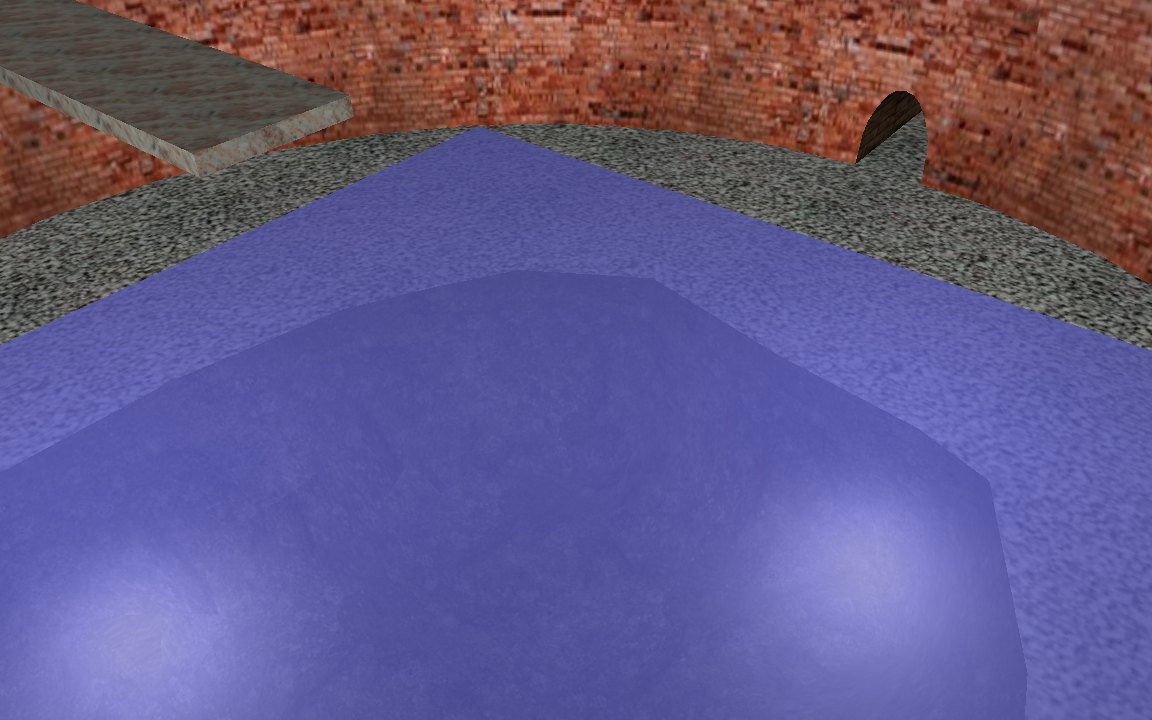
\includegraphics[width=2.3in]{water_shaders_0}
  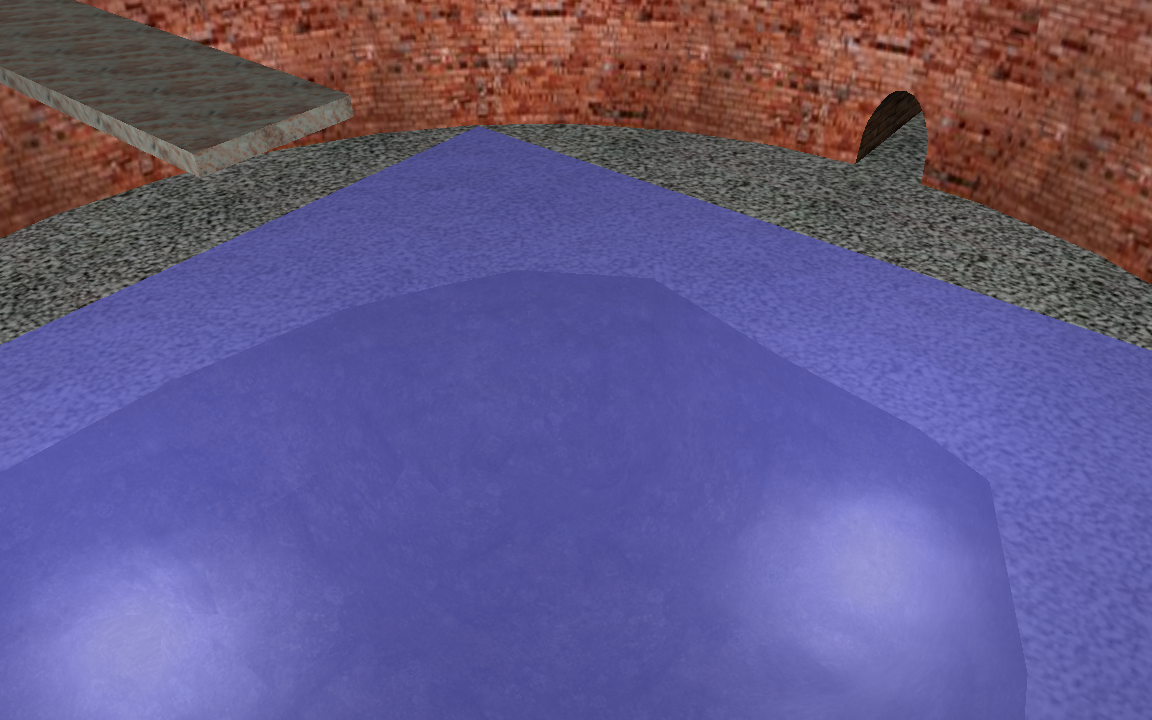
\includegraphics[width=2.3in]{water_shaders_1}
  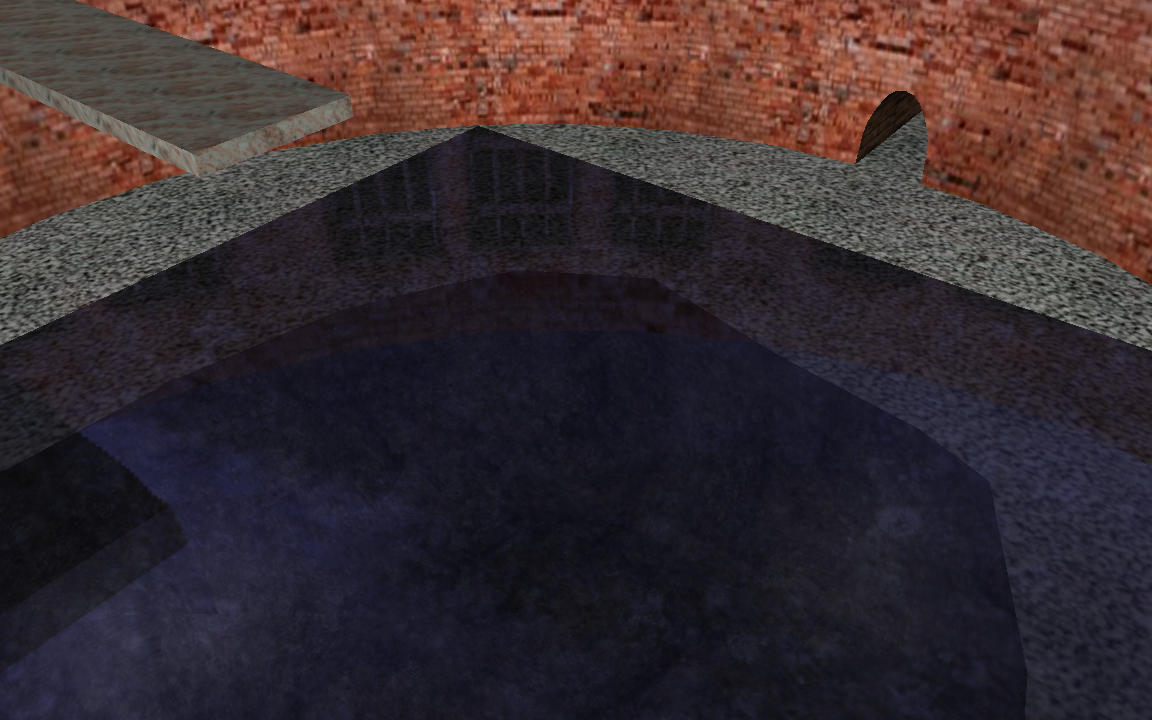
\includegraphics[width=2.3in]{water_shaders_2}
  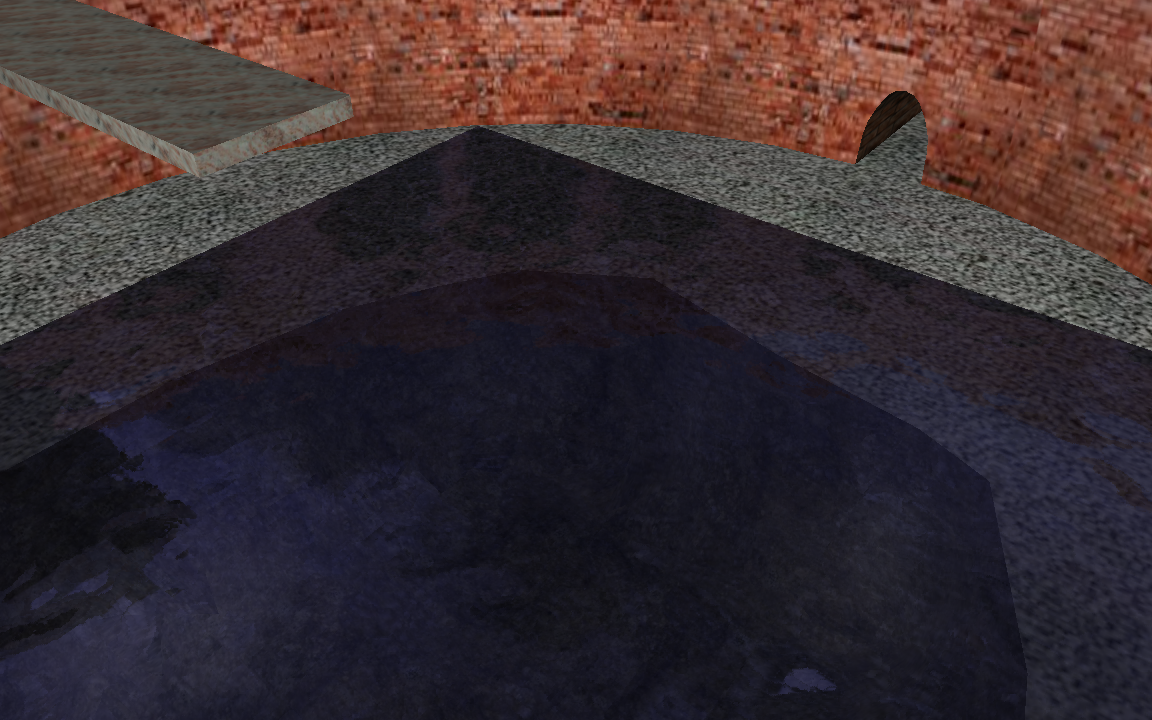
\includegraphics[width=2.3in]{water_shaders_3}
  \caption{Water using our effects: 1) Per-pixel lighting and bump mapping.
2) Per-pixel lighting and reflections and refractions (by a single environment cube map texture).
3) All effects.}
\end{figure*}

We can also wrap 2D and 3D noise inside a \texttt{ShaderTexture}.
A texture node like \texttt{NoiseTexture} from InstantReality
\myhref{http://doc.instantreality.org/documentation/nodetype/NoiseTexture/}{http://doc.instantreality.org/documentation/nodetype/NoiseTexture/}
may be implemented on GPU by a simple prototype using \texttt{ShaderTexture}.

\begin{figure}[H]
  \centering
  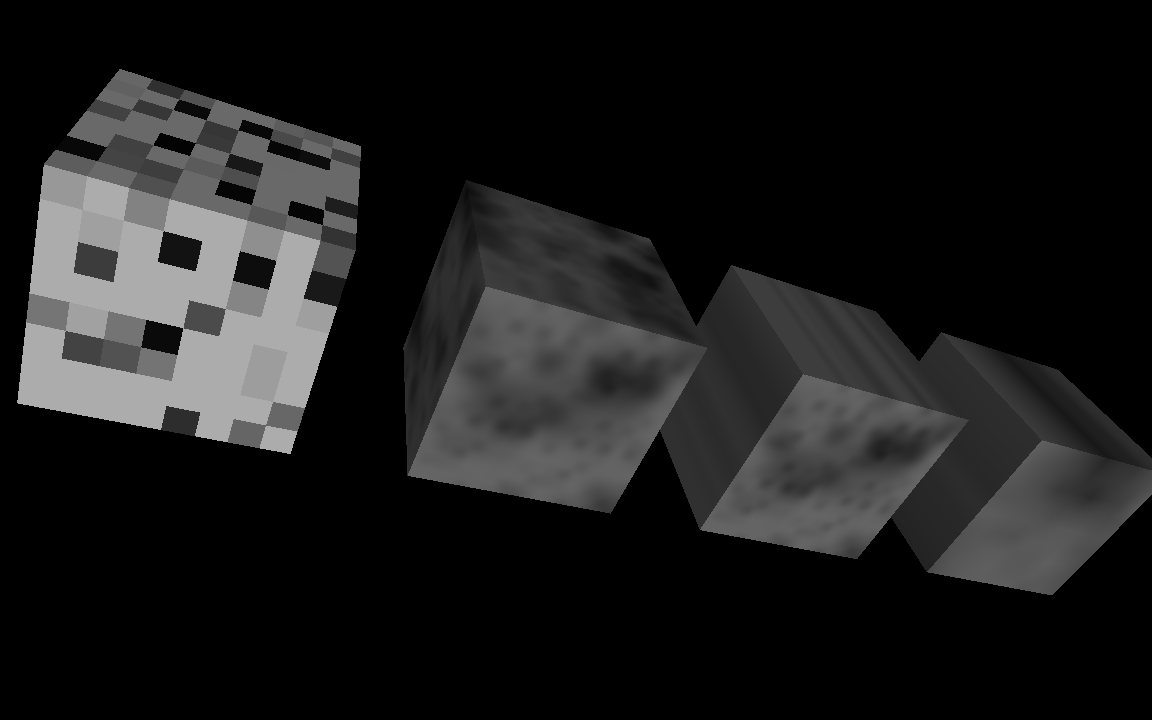
\includegraphics[width=3in]{noise}
  \caption{3D and 2D smooth noise on GPU, wrapped in ShaderTexture.}
\end{figure}

We would like to emphasize that all the effects demonstrated here
are theoretically already possible by using the X3D \textit{Programmable
shaders component} component.
However, actually implementing them is extremely cumbersome using this
standard component. You would first
have to prepare a shader code to calculate all the (multi-)texturing, lighting,
shadows, and all the other effects that you use in your scene.
This is a large work if you consider all the X3D options, and note that
a shader should remain optimized for a particular setting.
Moreover, you would have to calculate some global options,
like which light sources and fog nodes affect the given shape.
Effectively, this isn't really doable by a manual work --- instead
you would have to write a shader generator program. Our you could use
an existing shader generation system... which is exactly what our paper
is about. The implementation of our effects simply constructs and links
appropriate shader, gathering the information from all the nodes
that affect the given shape. And all the information is nicely integrated
with X3D nodes, effects are specified at suitable nodes, and their
uniform values and attributes are integrated with X3D fields.

\section{Short reference of available plugs}

TODO: maybe make it a table? We can probably waste 0.5-1 page on this
without a problem. Document this at the end, when everything is settled down.

For each plug:
- plug name
- declaration (parameter order and types must match)
- type (fragment or vertex)
- docs: called when?

specials:
texture\_color : has texture parameter only when not within ShaderTexture.
Texture parameter type corresponds to VRML/X3D node type (samplerXxx).

vertex\_object\_space, vertex\_object\_space\_change: you can change
only in the 1st one.

\section{Complete example models}

Examples are available inside our engine demo models on
\myhref{http://vrmlengine.sourceforge.net/kambi\_vrml\_test\_suite.php}{http://vrmlengine.sourceforge.net/kambi_vrml_test_suite.php}.
The relevant demos are mainly inside \texttt{compositing\_shaders},
also the \texttt{water} contains examples of the water implementation
using our effects.
You can checkout them from SVN, or just browse through a web browser,
using the URL
\myhref{https://vrmlengine.svn.sourceforge.net/svnroot/vrmlengine/trunk/kambi\_vrml\_test\_suite/compositing\_shaders/}{https://vrmlengine.svn.sourceforge.net/svnroot/vrmlengine/trunk/kambi_vrml_test_suite/compositing_shaders/}.

You can open the examples using any of our engine tools,
like \texttt{view3dscene} from
\myhref{http://vrmlengine.sourceforge.net/view3dscene.php}{http://vrmlengine.sourceforge.net/view3dscene.php}.

You can run \texttt{view3dscene} with \texttt{--debug-log-shaders} command-line
option. Output (stdout) will show you the final shader code generated,
and also the OpenGL log after linking shaders.
This is a useful way to learn about our shader rendering internals.

Another useful option to try in \texttt{view3dscene} is to switch to
\textit{View $->$ Shaders $->$ Enable For Everything} mode.
This will force shader rendering for all the shapes,
while by default we use shader rendering only for the shapes that
require particular effects (shaders by \texttt{ComposedShader}, effects
described in this paper, shadow maps and such).
Forcing shader rendering for everything allows to visually see
how our shaders implement the whole X3D lighting and texturing model.
It also makes the whole lighting calculation per-pixel, resulting
in particular in beautiful light spot highlights.

Development notes: only the SVN kambi\_vrml\_test\_suite contains
compositing\_shaders subdirectory.
You also have to use view3dscene from SVN or nightly builds,
see \myhref{http://michalis.ii.uni.wroc.pl/vrmlengine-snapshots/}{http://michalis.ii.uni.wroc.pl/vrmlengine-snapshots/}.

\bibliographystyle{acmsiggraph}
\nocite{*}
\bibliography{compositing_shaders}

\end{document}
